\documentclass[a4j,12pt,]{jarticle}
 \usepackage[dvipdfmx]{graphicx}
 \usepackage{float}
 \usepackage{siunitx} %%SI単位系用
 \usepackage{amssymb, amsmath}
 \usepackage{ascmac,here,txfonts,txfonts}
\usepackage{listings,jlisting}
\usepackage[dvipdfmx]{color}
\lstset{%
  language={Python},
  basicstyle={\small},%
  identifierstyle={\small},%
  commentstyle={\small\itshape\color[rgb]{0,0.5,0}},%
  keywordstyle={\small\bfseries\color[rgb]{0,0,1}},%
  ndkeywordstyle={\small},%
  stringstyle={\small\ttfamily\color[rgb]{1,0,1}},
  frame={tb},
  breaklines=true,
  columns=[l]{fullflexible},%
  numbers=left,%
  xrightmargin=0zw,%
  xleftmargin=3zw,%
  numberstyle={\scriptsize},%
  stepnumber=1,
  numbersep=1zw,%
  lineskip=-0.5ex%
}
\begin{document}

{\noindent\small 第13回報告書 \hfill\today}
\begin{center}
  {\Large 分布定数線路の周波数特性}
\end{center}
\begin{flushright}
  愛媛大学工学部 \\
  8531037m \\
  祖父江匠真 \\
\end{flushright}

\section{はじめに}

分布定数線路の周波数特性を調べた.

\section{分布定数線路の周波数特性}

図 \ref{p1}の同軸ケーブルの仕様表より, 3D-2Vケーブルの減衰特性の折れ線グラフを図 \ref{p2} に示す.

\begin{figure}[H]
  \begin{center}
    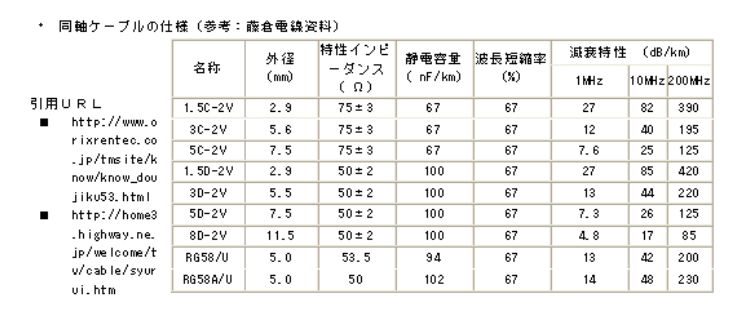
\includegraphics[width=160mm]{coaxial_cable_sheet.png}
    \caption{同軸ケーブルの仕様}
    \label{p1}
  \end{center}
\end{figure}

\begin{figure}[H]
  \begin{center}
    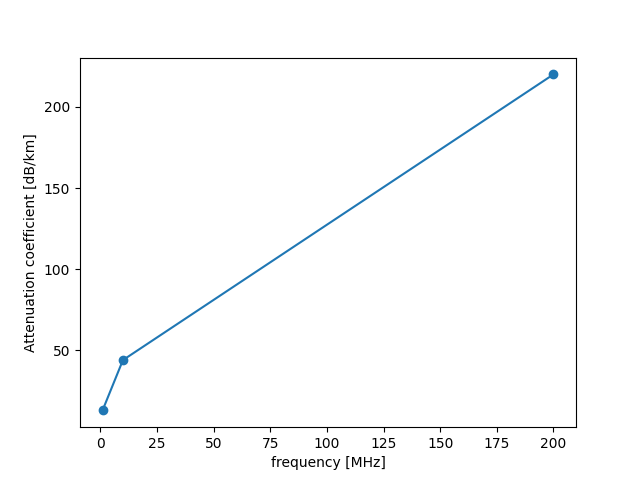
\includegraphics[width=140mm]{attenuation_coefficient.png}
    \caption{減衰特性の折れ線グラフ}
    \label{p2}
  \end{center}
\end{figure}

伝搬定数γ (= α + jβ)における減衰定数αについては, 図 \ref{p2} の周波数に対応した値を計算に用いた.

図 \ref{p3}の回路図について, 周波数特性を調べる.

\begin{figure}[H]
  \begin{center}
    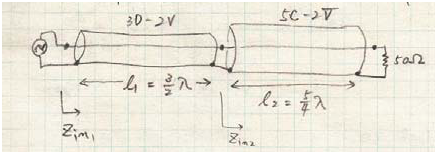
\includegraphics[width=140mm]{circuit.png}
    \caption{回路図}
    \label{p3}
  \end{center}
\end{figure}

Pythonで伝達関数の計算, 周波数特性のグラフを出力するプログラムをソースコード \ref{sc1}に示す.

\lstinputlisting[caption=周波数特性,label=sc1]{/home/sofue/lab/py/transferFunction.py}

ソースコード \ref{sc1} によって得られた周波数特性を図 \ref{p4} に示す.

\begin{figure}[H]
  \begin{center}
    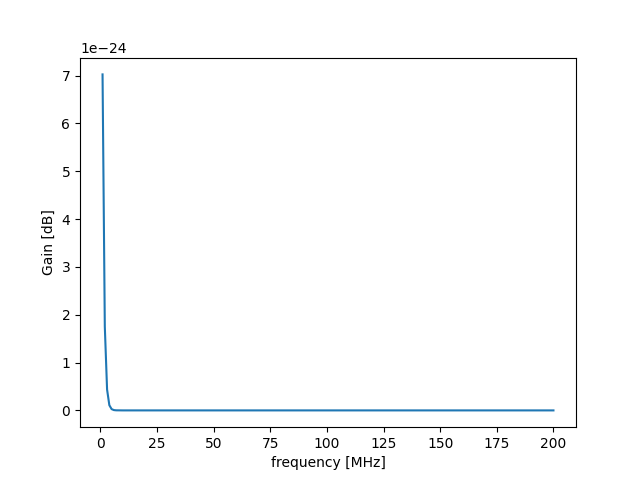
\includegraphics[width=140mm]{frequency_characteristic.png}
    \caption{周波数特性(1MHz \textasciitilde 200MHz)}
    \label{p4}
  \end{center}
\end{figure}

図 \ref{p4} より, 周波数が10MHzを超えた辺りからゲインが0になっているのでプロットする周波数の値域を1MHz \textasciitilde 10MHzに変更した物を図 \ref{p5} に示す.

\begin{figure}[H]
  \begin{center}
    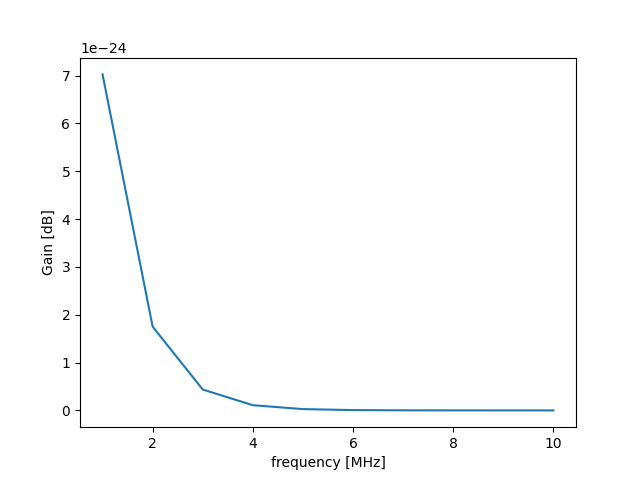
\includegraphics[width=140mm]{frequency_characteristic_1to10.png}
    \caption{周波数特性(1MHz \textasciitilde 10MHz)}
    \label{p5}
  \end{center}
\end{figure}

\section{おわりに}

今回は分布定数線路の周波数特性を調べたが, ローパスフィルターの周波数特性のようにはならなかった.

\begin{thebibliography}{5}
  \bibitem{1}都築,”2020Q4-応用通信工学II-都築”,moodle内,参照 October 20,2021.
\end{thebibliography}

\end{document}